% !TEX program = xelatex
\documentclass[UTF8,11pt,a4paper]{ctexart}

\usepackage{geometry}
\geometry{left=2.4cm,right=2.4cm,top=2.5cm,bottom=2.5cm}
\usepackage{amsmath,amssymb,mathtools}
\usepackage{booktabs,multirow,makecell,threeparttable,tabularx,array}
\usepackage{graphicx,float,caption,subcaption}
\usepackage{placeins}
\usepackage{xcolor}
\usepackage{enumitem}
\usepackage{tikz}
\usetikzlibrary{arrows.meta,positioning,shapes.geometric}
\usepackage[hidelinks]{hyperref}
\usepackage{microtype}

\captionsetup{font=small,labelsep=quad,skip=4pt}
\setlength{\parskip}{0.15em}
\setlength{\emergencystretch}{1.6em}
\linespread{1.32}
\setlist{nosep,leftmargin=2em}
\renewcommand{\arraystretch}{1.12}

\ctexset{
  section/format = \large\bfseries\raggedright,
  subsection/format = \normalsize\bfseries\raggedright,
}

\newcommand{\dd}{\mathrm{d}}
\newcommand{\deepflash}{\texttt{deepseek-flash}}
\newcommand{\deeppro}{\texttt{deepseek-v4-pro}}
\newcommand{\wpcond}{\texttt{word\_pairs}}
\newcommand{\basecond}{\texttt{baseline}}

\title{\heiti 先写 200 组词对能提升回答质量吗？\\[4pt]
\large ——对一项 240 对盲评实验的独立复算与再分析}
\author{作者姓名\textsuperscript{1}\\[3pt]
\small \textsuperscript{1} 单位名称，城市 邮编\\
\small \texttt{email@example.com}}
\date{}

\begin{document}
\maketitle

\begin{abstract}
\noindent
在问题前加一句“先输出 200 组两词短语，再从中获得灵感”，是中文大模型社区流行的一种“灵感注入”式提示。
本文对一个公开实验的 240 对盲评数据做独立复算与再分析。该实验覆盖 6 个开放式任务、2 个生成模型、2 个评委，
每个“任务 $\times$ 条件”单元重复 10 次。复算显示：直接回答在 224/240 对中获胜（93.3\%，任务聚类
bootstrap 95\% 置信区间 $[86.7\%, 97.1\%]$）；五个维度中仅原创性略升（$+0.31$），
逻辑性、具体性、可操作性与整体质量分别下降 $1.54$、$2.08$、$2.32$ 与 $1.72$ 分。
进一步分析表明，这一差距与输出长度高度相关（Spearman $\rho=0.585$）：词对条件的正文被压缩到
对照的 73\%（\deepflash）与 46\%（\deeppro），而输出 token 数反而增至 2.02 倍与 1.60 倍；
在长度比不低于 0.9 的子集（$n=28$）上，胜率降至 67.9\%；将长度差纳入回归后，等长处的条件效应
由 $-1.72$ 收窄至 $-0.82$（95\% CI $[-1.38, -0.26]$）。机制上，词对块中的词元只有 16.9\% 与 15.1\%
原样出现在正文中。本文认为，该提示的主要后果是输出预算的重新分配与正文压缩，而非“从词中获得灵感”；
据此提出等 token 预算、长度匹配与中性前缀对照三项设计修正。

\vspace{0.6em}
\noindent\textbf{关键词：}\ 提示工程；大语言模型；盲评；长度偏差；中介分析；可复现性

\vspace{0.9em}
{\small
\noindent\textbf{Abstract.}\ We independently recompute and re-analyze 240 blind pairwise comparisons from a public
experiment that asks a model to first emit 200 word pairs and then answer an open-ended task. Direct answers win
224/240 comparisons (93.3\%; task-clustered bootstrap 95\% CI $[86.7\%, 97.1\%]$). Only originality improves
($+0.31$); logic, concreteness, actionability and overall quality drop by $1.54$, $2.08$, $2.32$ and $1.72$ points.
The gap tracks answer length ($\rho=0.585$): answer bodies after removing the pair block are 73\% and 46\% as long as baselines while consuming
2.02$\times$ and 1.60$\times$ as many output tokens; restricting to length ratio $\ge 0.9$ reduces the baseline win rate
to 67.9\%, and a length-adjusted model puts the equal-length effect at $-0.82$ (95\% CI $[-1.38,-0.26]$). Only
16.9\% and 15.1\% of paired tokens reappear in the answer. We argue the prompt mainly reallocates output budget
rather than injecting inspiration, and propose equal-budget, length-matched and neutral-prefix controls.

\noindent\textbf{Keywords:}\ prompt engineering; large language models; pairwise judging; length bias;
mediation analysis; reproducibility
}
\end{abstract}

\vspace{0.4em}

%=====================================================================
\section{引言}
%=====================================================================

在中文大模型社区里流传着一种被称作“词对提示”的写法：在正式问题之前，要求模型先输出 200 组两词短语
（例如“晨光·缓存”“指纹·钥匙”“日志·折线”），再“从这些词中获得灵感”作答。支持者的直觉是，
随机的远距联想能把回答推离陈词滥调，产生更具原创性的方案。这个直觉并非空穴来风：心理学中的语义启动
（semantic priming）表明，先前的词汇加工会改变后续概念的通达性\cite{meyer1971}；而在语言模型上，
“先写出推理过程再给答案”也确实能在多步推理任务上带来稳定增益\cite{wei2022cot,kojima2022,Wang2023selfconsistency}。
但两者之间有一个关键差别：思维链的前置文本与答案共享同一套推理结构，其每一个中间步骤都被后续步骤使用；
词对与答案之间却只有极弱的语义关联，前置生成主要是消耗同一份输出预算。

这类“前置生成”提示究竟带来什么，目前缺少可复核的证据。已有的提示敏感性研究反复表明，提示的表面形式
——分隔符、格式、示例顺序、甚至与语义无关的模板——都可能显著改变模型表现\cite{sclar2024,webson2022,mizrahi2024}，
因此仅凭少量成功案例很难判断一个提示技巧的真实效应。与此同时，用大语言模型充当评委（LLM-as-a-judge）
虽然与人类偏好高度相关\cite{zheng2023}，却已知存在位置偏差\cite{wang2024fair}、冗长偏差\cite{saito2023,dubois2024lc}
与自我偏好\cite{panickssery2024}。当评测对象是“更短还是更长”这类系统性差异时，评委的打分很容易把
篇幅差异误读为质量差异。

本文不提出新的提示方法，而是对一个公开实验\footnote{数据与代码：\url{https://gitee.com/qwe12345678/jkdsfn}
（提交 \texttt{88e0b9a}，原 \texttt{v2-deepseek} 分支）。}做独立复算与再分析。该实验的原始结论是
“词对提示显著降低了回答质量”。我们复算后确认了胜负计数与五维均分，但认为这一表述把一个
“更短、更少细节”的差异包装成了“质量差异”，因而既高估了效应的普遍性，也错过了更有价值的机制问题。
本文的贡献是：

\begin{enumerate}[label=(\arabic*)]
\item \textbf{独立复算。}从原始 JSONL 重新计算全部胜负、五维评分、评委一致性与位置效应，
      与仓库自报数字逐项对齐，并给出任务聚类的置信区间，纠正了把 240 对当作 240 个独立样本导致的
      显著性高估（朴素二项检验 $p\approx4\times10^{-48}$，按任务聚类后 95\% CI 为 $[86.7\%, 97.1\%]$）。
\item \textbf{长度中介的定量证据。}通过分层、子集与含任务固定效应的回归，估计出长度差可解释约一半的
      评分差距；在长度相等处，条件效应由 $-1.72$ 收窄至 $-0.82$。
\item \textbf{机制证据。}给出“预算重分配”的直接测量：词对条件多花 60\%--102\% 的 token，却把正文压缩到
      46\%--73\%；同时词对词元在正文中的原样复现率仅 15\%--17\%，说明“灵感”在字面上几乎没有兑现。
\item \textbf{设计修正。}据此提出等 token 预算、长度匹配与中性前缀对照三项可操作的实验设计，
      并给出一份针对此类“前置生成”提示的效度清单。
\end{enumerate}

%=====================================================================
\section{相关工作}
%=====================================================================

\subsection{提示、推理与测试时计算}

让模型“先写点什么再回答”是提示工程中最常见的结构。思维链提示通过少量示例引导模型输出中间推理步骤，
在算术与常识推理上带来大幅提升\cite{wei2022cot}；零样本条件下，“让我们一步一步思考”也能触发类似行为\cite{kojima2022}；
自洽性方法进一步采样多条推理路径并投票\cite{Wang2023selfconsistency}。这些工作共享一个前提：
前置文本承载了可复用的中间结果。与之相对，测试时计算的扩展研究表明，增加采样或延长思考并不单调有益，
其收益取决于任务难度与验证器的质量\cite{snell2025}；对推理步长的分析也发现，步骤数与准确率之间并非
简单的正相关\cite{jin2024}。这提示我们：前置生成的价值不能由“写了更多”本身保证，而取决于写出来的内容
是否被后续过程真正利用。

\subsection{提示表面的敏感性}

另一条线索关注提示中与任务语义无关的表面特征。文献~\cite{webson2022} 发现，用无意义的模板替换自然语言指令后，
基于提示的模型表现下降有限，说明模型对指令“含义”的依赖弱于通常假设；文献~\cite{sclar2024} 系统量化了
分隔符、大小写、空格等格式扰动对性能的影响，发现其量级可与方法改进相当；文献~\cite{mizrahi2024} 则指出，
单提示评测的结论往往无法在提示集合上复现，呼吁多提示评测。这些结果共同说明：一个提示技巧的效应必须
在多任务、多模型、并有恰当对照的条件下测量，否则很容易把格式或预算的副作用记在“技巧”头上。

\subsection{LLM 评委的偏差}

以模型作为评委已成为开放生成任务的主要评测手段。MT-Bench 与 Chatbot Arena 的实验显示，
强模型评委与人类偏好的一致率可达 80\% 以上\cite{zheng2023}，但其偏差同样明确：交换 A/B 位置会改变结论\cite{wang2024fair}；
评委倾向偏好更长、更繁冗的回答\cite{saito2023}，这一偏差强到需要专门的长度控制方法才能在竞技场式评测中
得到可比胜率\cite{dubois2024lc}；评委还会识别并偏袒自己生成的文本\cite{panickssery2024}。
本文的实验恰好同时具备这三个风险源：条件之间系统性存在长度差、生成与评审来自同一模型家族、
且每个评委只评一次。

\subsection{语义启动的隐喻及其边界}

“词对”这一设计借用了心理学中语义启动的概念：先呈现一个词，会加快对语义相关词的加工\cite{meyer1971}。
但把这一现象迁移到自回归语言模型时需要谨慎。启动效应作用于\textbf{外部刺激的加工速度}，
而本文的条件作用于\textbf{同一段生成内部的上下文}：模型在写出 200 组词之后，这些词已经成为它自己的上文，
既可能提供联想线索，也可能挤占本应用于答案的位置。前者是“灵感”，后者是“开销”，
两者的净效应只能由实验区分——这正是本文要回答的问题。

\subsection{随机刺激与发散—收敛提示}

与“词对提示”最接近的先行工作分布在两条线上。第一条线是人类创造力方法。随机输入（random entry）
是水平思考的核心工具之一：刻意引入一个与问题无关的随机词、图像或物件，借远距联想把思考推离惯常的
方向\cite{debono1992}；其心理学基础可追溯到远距联想理论——创造过程即把语义距离较远的反应联结成
新颖而有用的组合\cite{mednick1962}。“词对提示”的直觉与这套方法几乎同构：200 组两词短语相当于
一次大规模的随机输入，只是执行者从人换成了模型，且联想过程被写进了答案所在的同一段输出。

第二条线是 LLM 提示研究。文献~\cite{taveekit2023rwb} 把随机词头脑风暴（random word brainstorming）
引入 ChatGPT 提示：把\textbf{外部}选定的随机词注入提示以激发非常规方案，问卷评估显示人类被试在
20 个问题中的 65\% 上更偏好该方法的产出。CREATIVEDC~\cite{nguyen2025creative} 则提出
“先发散、后收敛”的两阶段提示：模型先在同一次输出内头脑风暴一组非常规场景，再从中选取素材构造
编程练习，产出的高效用且互异任务数约为基线的 1.6 倍。后者与词对提示在结构上最为相近——前置的
发散文本与最终答案共享同一上下文与同一份输出预算——但其因变量是任务多样性而非盲评质量，
也未对两条件做预算或长度上的控制。

把这两条线放在一起，可以澄清本文的定位。其一，“用随机联想激发模型”并非新提议：它在创造力
工程中已有半个多世纪的历史，在 LLM 上也至少自 2023 年起就有正式研究；本文的增量不在提出该技巧，
而在于对它的社区流传变体（模型\textbf{自生成}词对、前置文本与答案\textbf{共享预算}）给出
可复核的负结果与机制解释。其二，先行工作的正面结论（新颖性偏好、多样性提升）与原实验的负面
结论（质量下降）表面上冲突，实则度量的是不同的因变量，且都缺少等预算、长度匹配与中性前缀
对照——这正是第~\ref{sec:design}~节三项设计修正试图补齐的缺口。

%=====================================================================
\section{实验与数据}
%=====================================================================

\subsection{设计与材料}

原实验采用 $6\times2\times10$ 的完全交叉设计：6 个开放式中文任务，2 个条件，每个单元重复 10 次。
任务覆盖“设计一门函数式编程语言”“低成本提升现有 LLM 性能”“面向独立开发者的 CLI 工具创意”
“提出一个新理论”“提出一个类九型人格/荣格八维的新模型”“提出一种新的机器学习架构”，
均属于没有唯一答案的开放式创意任务。两个条件只在提示前缀上不同：

\begin{itemize}
\item \basecond：直接给出任务提示；
\item \wpcond：在任务提示前加一句“在回答前面输出 200 组词，每组有两个词，从这些词获得灵感”。
\end{itemize}

表~\ref{tab:design} 汇总了实验配置。需要强调的是，两条件共享同一模型、同一温度（生成 0.6，清洗与评审 0.3）、
同一输出上限，唯一差别就是那句前缀，因此这是一个干净的单因素操纵。

\begin{table}[htbp]
\centering
\caption{实验配置}\label{tab:design}
\small
\begin{threeparttable}
\begin{tabular}{@{}ll@{}}
\toprule
项目 & 设置 \\
\midrule
任务 & 6 个开放式中文任务（见表~\ref{tab:task}） \\
条件 & \basecond（直接回答） vs.\ \wpcond（先写 200 组词对再回答） \\
重复 & 每“任务 $\times$ 条件”10 次 \\
生成模型 & \deepflash、\deeppro \\
评委 & 同上两个模型，交叉评审（$2\times2$ 共 4 格） \\
规模 & 240 条生成 / 120 条清洗 / 240 对盲评 \\
评分 & logic、concreteness、actionability、originality、overall，1--10 分 \\
位置平衡 & 按（生成模型、评委、任务、run）的确定性哈希决定 A/B 顺序，每对评一次 \\
清洗 & 由生成同款模型删除开头词对块与“第 $N$ 组”类引用，正则复查残留 \\
\bottomrule
\end{tabular}
\end{threeparttable}
\end{table}

\begin{table}[htbp]
\centering
\caption{六个任务及其提示语（节选）}\label{tab:task}
\small
\begin{tabular}{@{}clp{9.2cm}@{}}
\toprule
编号 & 简称 & 任务提示（原文节选） \\
\midrule
1 & 函数式语言 & 设计一个全新的函数式编程语言 \\
2 & 提升 LLM & 怎么低成本、不需要额外训练地大幅提升现有 LLM 的性能 \\
3 & CLI 工具 & 给出适合独立开发者开发 CLI 工具的一个 Idea \\
4 & 新理论 & 提出一个新的理论 \\
5 & 人格模型 & 提出一个新的类似于九型和荣格八维的模型 \\
6 & ML 架构 & 提出一个新的机器学习架构 \\
\bottomrule
\end{tabular}
\end{table}

\subsection{清洗与盲评}

\wpcond 的原始输出以词对块开头，若直接与 \basecond 比较，评委看到的将是“词对 + 答案”对“答案”，
差异会被词对块本身的篇幅主导。为此原实验引入清洗步骤：由同一模型删除词对块及正文中对词对的引用
（如“从上面词对中”“第 12 组”），得到 \texttt{cleaned} 文本，再用正则检查是否仍有编号或指代残留。
复算显示 120 条清洗结果全部无残留，清洗后文本与清洗前正文（原始输出去掉词对块后的部分）
的长度比中位数为 0.99，均值 0.979，最小 0.635——即清洗基本是“删掉词块 + 轻度改写”，
个别样本存在较大幅度删改。

盲评阶段，评委看到两段匿名文本 A 与 B，被要求按五个维度各打 1--10 分，并给出胜负与理由。
五个维度的操作化定义为：逻辑性（论证是否自洽、结构是否清楚）、具体性（是否有具体方案、参数与例子）、
可操作性（读者能否照着实施）、原创性（是否给出新颖的视角或组合）、整体质量（综合判断）。
评委以 JSON 输出胜负（A/B/tie）与一段自由文本理由，温度为 0.3，每对只评一次、不做多次采样平均。
需要说明的是，五个维度并不正交，整体质量与其余四维高度相关；因此本文以整体质量为主结果，
其余维度用于解释差异来源，而不单独作为“独立假设”检验。
A/B 顺序由确定性哈希决定，每条记录保存了 \texttt{swap}、\texttt{A\_source}、\texttt{B\_source}，
因此事后可以把分数还原到条件，也可以分解位置效应。这一点在原仓库中做得比多数同类实验规范。

\subsection{数据完整性与分析口径}

我们从仓库的 8 个 JSONL 文件（2 个生成模型 $\times$ 4 类记录）重算，未使用仓库自带的汇总文件。
所有阶段均为追加式写入，重复记录按 \texttt{(task\_id, condition, run)} 或 \texttt{(task\_id, run)}
取最新有效记录；生成 240 条（每模型 120 条）、清洗 120 条、盲评 240 对，无缺失、无重复。

全文统一记号：$\Delta$ 表示“词对条件 $-$ 直接回答”，故 $\Delta<0$ 表示词对条件更差；
除表~\ref{tab:budget} 的生成侧统计外，长度一律指评委实际看到的字符数
（\texttt{baseline\_content} 与 \texttt{cleaned\_content} 的长度），而非模型原始输出。统计上，我们把 6 个任务视为 6 个簇：由于同一任务内的 40 对共享同一提示，
它们并不独立，因此主结果报告按任务重抽样的聚类 bootstrap（$B=10\,000$）置信区间，
并辅以任务层面的符号检验；回归模型均含任务固定效应与任务聚类稳健标准误。
所有分析脚本与中间结果随文提供，可一键复现。

%=====================================================================
\section{结果}
%=====================================================================

\subsection{主效应：直接回答的压倒性优势}

240 对盲评中，直接回答胜 224 对，词对条件胜 15 对，平 1 对，胜率 93.3\%。
四个“生成模型 $\times$ 评委”格子的方向完全一致（表~\ref{tab:main}），
从 52/60 到 59/60 不等。格子之间的差异本身也有信息：以 \deeppro 为生成模型的两格几乎完全相同
（均为 59:1），而以 \deepflash 为生成模型的两格分别为 54:5 与 52:8——同一批文本换一个评委，
词对条件的胜场就从 5 变成 8。这说明受损程度首先取决于生成模型如何分配预算，评委的宽严只带来二阶波动。按任务聚类后，胜率的 95\% 置信区间为 $[86.7\%, 97.1\%]$，
$\Delta_{\text{overall}}$ 的均值为 $-1.72$，95\% CI $[-2.04, -1.38]$。
六个任务无一例外地偏向直接回答，符号检验的双侧精确 $p=0.031$。
作为对照，若错误地把 240 对视为独立样本，二项检验会给出 $p\approx4\times10^{-48}$——
这一数量级的差异正是聚类校正的意义所在。

\begin{table}[htbp]
\centering
\caption{主结果：四格胜负与分差（$N=240$）}\label{tab:main}
\small
\begin{threeparttable}
\begin{tabular}{@{}lrrrrrr@{}}
\toprule
\multirow{2}{*}{格子（生成 / 评委）} & \multirow{2}{*}{$n$} & \multicolumn{3}{c}{胜负} & \multirow{2}{*}{$\Delta_{\text{overall}}$} & \multirow{2}{*}{$\Delta_{\text{orig.}}$} \\
\cmidrule(lr){3-5}
 & & 直接 & 词对 & 平 & & \\
\midrule
\deepflash{} / \deepflash{} & 60 & 54 & 5 & 1 & $-1.27$ & $+0.52$ \\
\deepflash{} / \deeppro{}  & 60 & 52 & 8 & 0 & $-1.05$ & $+0.65$ \\
\deeppro{} / \deepflash{}  & 60 & 59 & 1 & 0 & $-2.38$ & $-0.22$ \\
\deeppro{} / \deeppro{}    & 60 & 59 & 1 & 0 & $-2.18$ & $+0.30$ \\
\midrule
合计 & 240 & 224 & 15 & 1 & $-1.72$ & $+0.31$ \\
\bottomrule
\end{tabular}
\begin{tablenotes}\footnotesize
\item 注：$\Delta$ 为“词对条件 $-$ 直接回答”的均分差。胜率 93.3\%，任务聚类 bootstrap 95\% CI $[86.7\%, 97.1\%]$。
\end{tablenotes}
\end{threeparttable}
\end{table}

\begin{figure}[htbp]
\centering
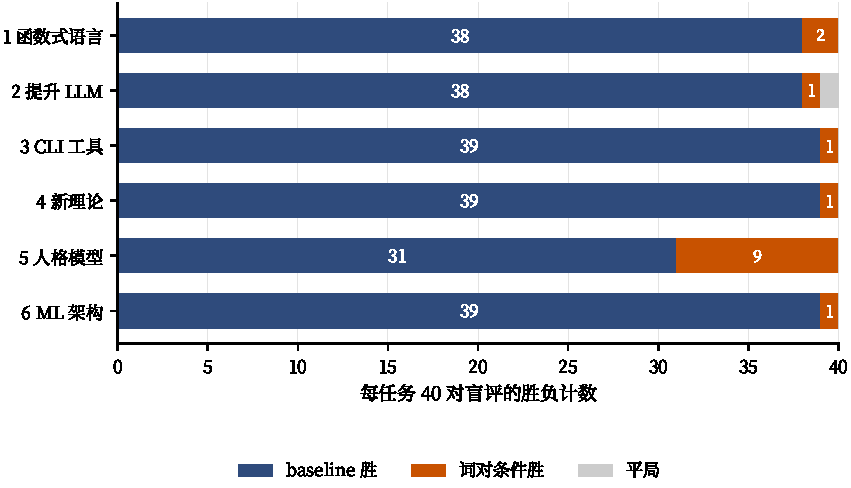
\includegraphics[width=0.92\textwidth]{figs/fig_wins_by_task.pdf}
\caption{分任务胜负分布（每任务 40 对）。任务 5“人格模型”是唯一出现较多词对胜场的任务。}\label{fig:task}
\end{figure}

\subsection{维度分解：只赢在原创性}

表~\ref{tab:dims} 与图~\ref{fig:dims} 把五维评分还原到条件后合并 240 对。词对条件在四个维度上全面落后：
可操作性 $-2.32$、具体性 $-2.08$、整体质量 $-1.72$、逻辑性 $-1.54$，
唯一为正的是原创性 $+0.31$（$d_z=0.25$）。分生成模型看，原创性收益主要来自 \deepflash（$+0.58$），
\deeppro 上几乎为零（$+0.04$）——这与“词对能稳定提升创造力”的说法不符，说明该收益依赖生成模型。

从效应量看，四个负向维度的 $d_z$ 在 $-1.25$ 至 $-1.48$ 之间，按常规标准属于大效应。但这一数值
部分来自评分尺度的天花板：直接回答的均分已接近 9 分，质量下降被压缩在高分区间内，
因而 $d_z$ 同时混合了“真实下降”与“尺度非线性”两种成分，不宜与心理学实验中的效应量直接类比。
原创性的 $d_z=0.25$ 处于小效应区间；在只有 6 个簇、且评委只评一次的条件下，其不确定性很大，
本文只把它当作方向性证据，而不据此主张“词对能提升创造力”。

\begin{table}[htbp]
\centering
\caption{五维评分：条件均值与配对效应量（$N=240$）}\label{tab:dims}
\small
\begin{tabular}{@{}lrrrr@{}}
\toprule
维度 & 直接回答 & 词对条件 & $\Delta$ & Cohen's $d_z$ \\
\midrule
逻辑性 logic & 8.98 & 7.44 & $-1.54$ & $-1.25$ \\
具体性 concreteness & 8.90 & 6.83 & $-2.08$ & $-1.36$ \\
可操作性 actionability & 8.67 & 6.35 & $-2.32$ & $-1.48$ \\
原创性 originality & 7.54 & 7.85 & $+0.31$ & $+0.25$ \\
整体质量 overall & 8.83 & 7.11 & $-1.72$ & $-1.36$ \\
\bottomrule
\end{tabular}
\end{table}

\begin{figure}[htbp]
\centering
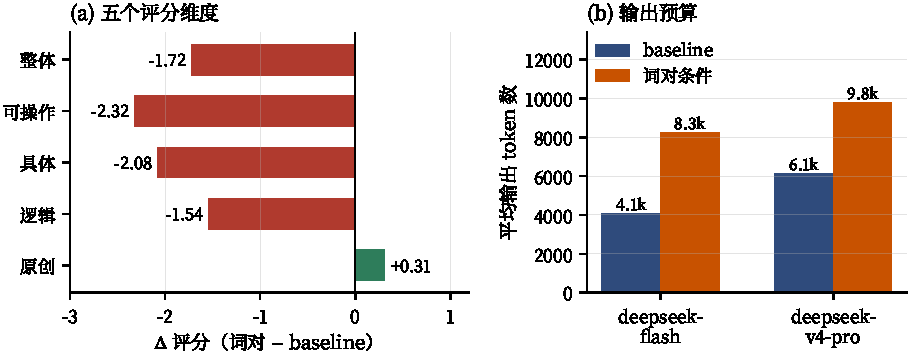
\includegraphics[width=0.95\textwidth]{figs/fig_dims_budget.pdf}
\caption{(a) 五个维度的均分差；(b) 两条件的平均输出 token 数。词对条件多花 60\%--102\% 的预算，
却在四个质量维度上同时下降。}\label{fig:dims}
\end{figure}

\subsection{任务异质性：发散任务更受益}

图~\ref{fig:task} 显示，五个任务的直接回答胜率都不低于 95\%，唯独任务 5“人格模型”为 77.5\%
（31:9）。这一差异有直观解释：提出一个类九型人格的模型需要在多个心理维度间做类比与组合，
词对提供的远距联想恰好能充当素材；而“设计一门编程语言”“提出一个新理论”这类任务有较强的
内在结构要求，压缩后的正文更容易丢掉定义、机制与可检验预测。也就是说，词对条件并非在所有任务上
同等有害，其收益与代价取决于任务对“发散联想”和“结构细节”的相对需求。
任务 5 也是任务内长度—分数相关最高的一格（$\rho=0.89$，$\rho^2\approx0.79$）：该任务的评分高度由篇幅决定，
因此它虽然最“受益”，胜率也只是从其余五个任务的平均 96.5\% 降到 77.5\%，并未真正翻转。

\subsection{关键发现：长度是主要通道}

表~\ref{tab:len} 按“清洗后正文长度 / 直接回答长度”分层。词对条件的胜率随长度比单调上升：
长度比低于 0.5 的 100 对中直接回答全胜；长度比高于 1.2 的 8 对中词对条件胜 6 对。
把长度比不低于 0.9 的 28 对单独取出，胜率从 93.3\% 降至 67.9\%，平均分差从 $-1.72$ 收窄到 $-0.50$；
若要求清洗后正文至少与直接回答等长（$n=18$），胜负变为 9:9，平均分差 $-0.22$。
在 $\pm15\%$ 的长度带内（$n=26$），胜率仍有 76.9\%，但分差已降至 $-0.65$。
240 对的 Spearman 相关为 $\rho=0.585$（$p<2\times10^{-23}$），逐格相关约在 0.30--0.50 之间，方向一致。
把样本按任务切开分别计算，$\rho$ 落在 0.37--0.89 之间（中位 0.56），六个任务全部为正且
$p<0.02$——这说明长度效应不是某一两个任务造成的伪影，而是贯穿整个任务集的稳定结构。

\begin{table}[t]
\centering
\caption{按长度比分层的胜负与分差}\label{tab:len}
\small
\begin{tabular}{@{}lrrrrr@{}}
\toprule
长度比区间 & $n$ & 直接胜 & 词对胜 & 平 & $\Delta_{\text{overall}}$ \\
\midrule
$<0.5$      & 100 & 100 & 0 & 0 & $-2.50$ \\
$0.5$--$0.8$ & 96 & 92 & 4 & 0 & $-1.36$ \\
$0.8$--$1.0$ & 26 & 23 & 2 & 1 & $-1.08$ \\
$1.0$--$1.2$ & 10 & 7 & 3 & 0 & $-0.70$ \\
$>1.2$      & 8 & 2 & 6 & 0 & $+0.38$ \\
\midrule
子集：长度比 $\ge0.9$ & 28 & 19 & 9 & 0 & $-0.50$ \\
子集：长度比 $\ge1.0$ & 18 & 9 & 9 & 0 & $-0.22$ \\
子集：$|\text{长度比}-1|\le0.15$ & 26 & 20 & 5 & 1 & $-0.65$ \\
\bottomrule
\end{tabular}
\end{table}

\begin{figure}[t]
\centering
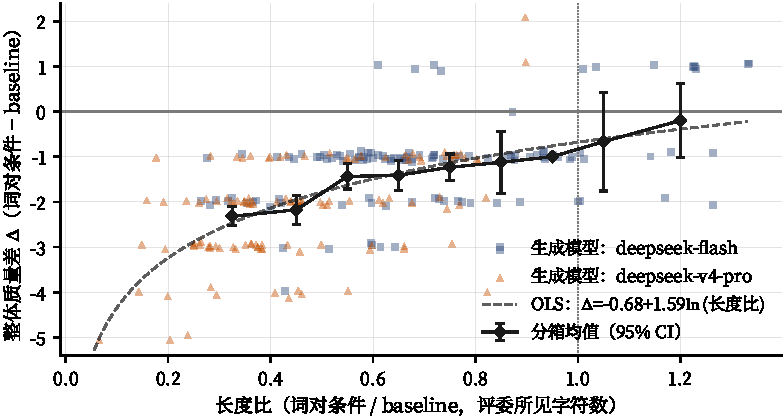
\includegraphics[width=0.9\textwidth]{figs/fig_len_score.pdf}
\caption{长度比与整体质量差的关系。散点为 240 对，黑线为分箱均值（95\% CI），
虚线为 $\Delta=a+b\ln(\text{长度比})$ 的最小二乘拟合。}\label{fig:len}
\end{figure}

图~\ref{fig:len} 把 240 个点与分箱均值画在一起。可以看到两点：其一，分箱均值几乎落在一条对数曲线上，
说明长度与评分的关系是连续而非阈值式的；其二，即便在长度比接近 1 的位置，均值仍在零线以下，
提示长度并非唯一通道。

为给出可解释的定量结论，我们拟合含任务固定效应的回归
$\Delta_{\text{overall}}=\alpha+\beta\ln(L_{\text{wp}}/L_{\text{base}})+\gamma_{\text{task}}+\varepsilon$，
标准误按任务聚类。结果为 $\beta=1.65$（$SE=0.30$，$t=5.42$，$\mathrm{df}=5$，$p=0.003$），
$\alpha=-0.82$（95\% CI $[-1.38, -0.26]$）。斜率可读作“长度比每提高一个自然对数单位（即乘以 $e$），分差改善 1.65 分”；
截距则给出\textbf{长度相等时仍残留的条件差异}，其绝对值约为原始均值差 $-1.72$ 的 48\%。
也就是说，长度差大致解释了一半的评分差距，另一半来自长度之外的因素。

这里需要明确因果语言。长度不是普通混杂变量，而是\textbf{处理后变量}（post-treatment mediator）：
条件影响长度，长度又影响评分。对中介变量分层或回归，得到的是“若长度被固定，效应会是多少”的反事实估计，
而不是无偏的因果效应；若还存在同时影响长度与评分的未观测因素（例如模型在长任务上的“耐心”），
估计仍可能有偏。因此本文的结论是“长度是主要通道之一，约解释一半”，而不是“词对没有效果”。
剩余的那一半，一部分可能来自清洗过程中被删掉的细节，一部分来自词对条件本身更差的组织结构——
后文的文本特征分析支持这一解读。

\FloatBarrier
\subsection{预算重分配：多花一倍 token，写得更短}

表~\ref{tab:budget} 给出生成侧的测量。词对条件的平均输出 token 在 \deepflash{} 上为
4\,090$\to$8\,252（2.02 倍），在 \deeppro{} 上为 6\,123$\to$9\,796（1.60 倍），
但去除词对块后的正文只有对照的 73\% 与 46\%。词对块本身约 2\,290--2\,440 字符，
相当于一篇直接回答的 68\%--82\%；换言之，模型把相当一部分输出预算花在了与答案无关的清单上。

\begin{table}[t]
\centering
\caption{输出预算与正文长度（每条件 60 条）}\label{tab:budget}
\small
\begin{tabular}{@{}lrrrr@{}}
\toprule
\multirow{2}{*}{指标} & \multicolumn{2}{c}{\deepflash} & \multicolumn{2}{c}{\deeppro} \\
\cmidrule(lr){2-3}\cmidrule(lr){4-5}
 & 直接回答 & 词对条件 & 直接回答 & 词对条件 \\
\midrule
平均输出 token & 4\,090 & 8\,252 & 6\,123 & 9\,796 \\
平均输出字符 & 2\,774 & 4\,318 & 3\,576 & 4\,090 \\
其中正文平均字符 & 2\,774 & 2\,031 & 3\,576 & 1\,653 \\
正文 / 直接回答 & 1.00 & 0.73 & 1.00 & 0.46 \\
词对条数（均值） & -- & 199.9 & -- & 192.3 \\
词元原样复现率 & -- & 16.9\% & -- & 15.1\% \\
触及输出上限条数 & 0 & 1 & 0 & 2 \\
\bottomrule
\end{tabular}
\end{table}



值得强调的是，缩短并非被动截断。从观测值看，两个条件的输出上限相同（最大输出为
16\,383/16\,384 个 token）。120 条词对输出中只有 3 条真正触顶，且这 3 条都缺少收尾标点；另有 1 条未触顶、
同样没有收尾标点，其余 116 条都以正常标点结束。
也就是说，模型在写完词对之后，\textbf{主动}把答案压缩了：它仍有预算，但选择了更短的答复。
这与“预算不足”不同，更像一种自我节流——模型把“已经写了很多”当成了停止的理由。
这一机制也解释了为什么 \deeppro 受损更重：它的词对块更长、正文压缩更狠（0.46），
对应的分差也更大（$-2.28$ 对 $-1.16$）。

\FloatBarrier
\subsection{机制检验：词对真的被“用上”了吗}

如果词对的作用是“提供灵感”，那么词对中的词应当以某种形式进入正文。我们把词对块中的 2--4 字中文词元
与英文词抽取出来，检查其是否原样出现在正文中（这是覆盖率的下界，忽略改写、同义与词形变化）。
结果为：\deepflash 平均 16.9\%（中位 14.0\%，最高 50.9\%），\deeppro 平均 15.1\%（中位 13.3\%，最高 73.2\%）。
即便按最宽松的口径，也有八成以上的词没有被使用。

词对的排版也提示处理并未标准化：两个模型都混用“每行一组”（如“1. 终端·灵感”）与
“每行十组、以分号分隔”，\deeppro 还出现“三位补零（001.）”“【1--10】分块”等格式，合计至少四种。
这不影响本文的结论，但它意味着任何按行计数的剂量校验都会严重低估词对数量；若后续研究要复核处理强度，
必须在生成时就记录 \texttt{pair\_count}，而不是事后用正则去猜。

与之对照，200 组词对基本都写满了
（前者全部 $\ge191$ 组，后者 58/60 达到 190 组以上），说明模型并未偷工减料，
低复现率不是因为词没写出来，而是因为写出来的词大多与后续答案无关。

把这一结果与上一节合起来看，词对条件的因果链条更像是：
\textbf{前置清单占用预算} $\rightarrow$ \textbf{正文被压缩} $\rightarrow$ \textbf{细节与结构减少} $\rightarrow$ \textbf{评分下降}，
而不是“词对激发联想 $\rightarrow$ 答案更有创意”。原创性上的小幅提升说明前者并非完全没有副产物，
但其量级（$+0.31$，且仅在一个生成模型上成立）远不足以抵消其他维度的损失。

\subsection{评委行为：位置、宽严与天花板}

用 $2\times2$ 分解可以把评委看到的差异拆成条件效应与位置效应：
当 A 为直接回答时，$A-B$ 的均值为 $+2.12$；当 A 为词对条件时，$A-B$ 为 $-1.37$。
由此得到条件效应 $+1.74$、位置效应 $+0.37$。位置偏差存在但不是主因；
不过由于 A/B 顺序由哈希而非分层平衡决定，直接回答落在 A 位的对数为 113/240，位置与样本并不完全独立，
这一点会放大噪声。

两位评委的一致性也值得注意。对 \deepflash 的 60 对，两位评委一致 52 对（86.7\%），
Cohen's $\kappa=0.36$，属于弱一致；对 \deeppro 的 60 对，一致性为 100\%，$\kappa=1.00$——
但这个“完美一致”建立在边际分布极度失衡（59:1）之上：60 对中只有 1 对由词对条件获胜，
正例过少，$\kappa=1.00$ 不足以证明评委可靠。两位评委的宽严差异其实不大，被评文本的差异更明显：
\deepflash 作为评委时，对 \deepflash 与 \deeppro 文本的五维均分为 8.09 与 7.46；
\deeppro 作为评委时为 8.22 与 7.63。约 0.6 分的差距来自被评文本
（同一评委评 \deepflash 文本比评 \deeppro 文本高约 0.6 分），评委之间的差异只有 0.13--0.17 分。
这意味着绝对分数仍不宜跨评委直接比较，只有同一评委内的相对比较才完全可比。

评分还明显存在天花板效应（图~\ref{fig:score}）：480 个整体分中，9 分 216 个（45\%）、8 分 128 个，
10 分仅 2 个，均值 7.97、标准差 1.26。分布集中在高分段会压缩区分度，
也会让“某一维度略高”这类小效应更难被可靠检出。评审理由的关键词统计同样指向篇幅：
在 240 条理由中，“可操作”出现于 184 条、“结构”168 条、“具体”158 条、“完整”148 条、“清晰”144 条、“细节”140 条——
评委在解释自己的偏好时，反复使用的正是短答案最容易缺失的属性。

\begin{figure}[htbp]
\centering
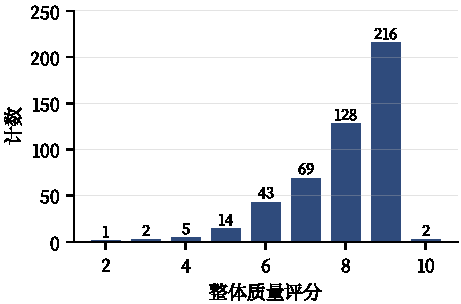
\includegraphics[width=0.52\textwidth]{figs/fig_score_dist.pdf}
\caption{480 个整体质量评分的分布。45\% 为 9 分，天花板效应明显。}\label{fig:score}
\end{figure}

\subsection{文本特征：评分在追踪什么}

为验证“评分随篇幅与结构走”的判断，我们抽取了若干与长度相关的客观特征，计算其条件间差值与
$\Delta_{\text{overall}}$ 的 Spearman 相关：字符数 0.541、段落数 0.480、标题数 0.441、
数字个数 0.357、加粗片段 0.236、列表项 0.201。以标准化特征差与任务固定效应做多元回归，
字符数（$\beta=0.84$，$SE=0.28$）与标题数（$\beta=0.17$，$SE=0.05$）显著为正，
代码块数为负（$\beta=-0.25$，$SE=0.08$），$R^2=0.47$。也就是说，近一半的评分方差可以由
“答案变短了多少、结构少了多少”解释。这与 LLM 评委的冗长偏差文献一致\cite{saito2023,dubois2024lc}，
但在本文中它不只是评测噪声：词对条件确实系统性地删掉了细节与结构，评委的偏好与文本的实际变化方向相同，
两者叠加，才产生了 93\% 的胜率。

\subsection{跨代复现：v1 的方向一致、量级更小}

同一仓库还包含一代更早的实验（v1）：使用 \texttt{moonshotai/kimi-k3} 作为生成与评审模型，
每格 10 次、共 60 对。复算结果（表~\ref{tab:v1v2}）为 49:10:1（直接回答胜率 81.7\%），五维方向与 v2 完全一致
（整体 $-1.03$、可操作性 $-1.65$、原创性 $+1.10$）。更有意思的是长度：v1 的清洗后正文为对照的 84.1\%，
远没有 v2 那么极端；相应的胜率也更低（81.7\% 对 93.3\%），长度—分数相关为 $\rho=0.359$，
在长度比不低于 0.9 的 17 对上胜率降至 64.7\%。

\begin{table}[htbp]
\centering
\caption{两代实验的对照：长度压缩越强，胜率差距越大}\label{tab:v1v2}
\small
\begin{tabular}{@{}lll@{}}
\toprule
项目 & v1（Kaggle） & v2（本地，本文主分析） \\
\midrule
生成 / 评审模型 & kimi-k3 / 同模型 & \deepflash{} 与 \deeppro{} 交叉评审 \\
有效对数 & 60 & 240 \\
胜负（直接:词对:平） & 49:10:1 & 224:15:1 \\
直接回答胜率 & 81.7\% & 93.3\% \\
$\Delta_{\text{overall}}$ & $-1.03$ & $-1.72$ \\
$\Delta_{\text{originality}}$ & $+1.10$ & $+0.31$ \\
清洗后正文长度比（均值） & 0.841 & 0.585 \\
Spearman $\rho$（长度比, $\Delta$） & 0.359 & 0.585 \\
长度比 $\ge0.9$ 子集胜率 & 64.7\%（$n=17$） & 67.9\%（$n=28$） \\
\bottomrule
\end{tabular}
\end{table}

两代实验构成一个有用的准实验对照：设计相同、模型不同，长度压缩的程度不同，胜率也随之不同，
且方向一致。这与“长度是主要通道”的解释相容。当然，两代实验在任务措辞、评委数量、运行环境上也有差异，
不能当作严格的剂量—反应证据，但它至少说明：把 v2 的 93\% 当作“词对提示的一般性质”是危险的，
它更像是“某个模型在某个预算下把答案压缩到 46\%--73\% 之后的结果”。

%=====================================================================
\section{讨论}
%=====================================================================

\subsection{为什么原创性上升、其余维度下降}

一个自然的解释是：词对提供的是\textbf{远距概念并置}（如“缓存·沙漏”“日志·折线”），
这类并置会诱导比喻与跨域映射，从而在“新颖性”上得分；但它不提供定义、机制、边界条件与可执行步骤，
而这些恰是逻辑性、具体性与可操作性的来源。更关键的是，写词对消耗了预算，模型在剩余篇幅内只能给出
压缩版方案——压缩首先删掉的就是细节与限定条件。于是出现一个看似矛盾、实则自洽的模式：
答案“更有想法”，但“更不像一个能落地的方案”。任务 5（人格模型）的损失之所以较小，是因为该任务本就以
类比与维度组合为核心，压缩带来的损失较小，而联想带来的收益较大。

\subsection{“灵感注入”叙事的三处反证}

把本文的证据放在一起，可以对“词对提示能注入灵感”给出三条独立的反证。
第一，\textbf{吸收率低}：词对中的词元只有 15\%--17\% 原样进入正文，八成以上的“灵感素材”没有被使用。
第二，\textbf{预算明显增加}：词对条件平均多花 60\%--102\% 的 token，如果灵感真的有效，
这笔投入应当换来更好的答案，而不是更短的答案。第三，\textbf{等长后效应大幅缩水}：
在长度相近的子集上，胜率从 93\% 降到 68\%，等长点的条件效应只剩 $-0.82$。
三条证据指向同一个结论：该提示的主要作用是改变输出的\textbf{预算分配}，而不是改变模型的\textbf{知识或联想}。

\subsection{对提示设计的启示}\label{sec:design}

如果确实想利用“远距联想”，本文的结果提示三种更合理的做法。
其一，\textbf{把联想放在答案之后}：先让模型给出完整方案，再让它用词对做“二次发散”，最后合并修订；
这样联想不占用首轮答案的预算。其二，\textbf{拆成两次调用}：一次生成词对，一次在独立上下文中作答，
并把词对作为可选的参考材料而非必须前置的清单；这样可以用“是否引用”来度量收益。
其三，\textbf{控制预算}：给对照组同样的 token 上限与“写到 X 字”的中性指令，使两条件的预算对称。
无论采用哪种做法，都应当加入\textbf{中性前缀对照}——例如 200 行无意义文本或 200 组随机词——
以区分“联想”与“仅仅多写了一段”。

如果研究目标确实是“验证联想”，更合适的做法是把因变量从“答案质量”换成“联想的使用”：
统计词对词元在正文中的出现率与位置、要求模型显式标注“由第 $k$ 组词启发”，
或由人工判断某个比喻是否真的来自词表。本文的覆盖率指标只是这种测量的最粗版本，
但它已足以说明：在这批数据里，“灵感”不是主要通道。

\subsection{对评测的启示}

本文的分析也说明，开放生成任务的 A/B 评测需要三项最低限度的防护。
第一，\textbf{报告并控制长度}：至少报告两条件的长度分布，并在长度匹配的子集上复算胜率；
条件允许时应使用长度控制的胜率\cite{dubois2024lc}。第二，\textbf{按簇做推断}：同一提示下的多次采样
不是独立样本，应按任务（或提示）做聚类 bootstrap，否则 $p$ 值会被严重低估、显著性被高估几十个数量级。
第三，\textbf{评委独立}：至少引入一个非生成家族的评委，并对每对做双向评审，
报告 $\kappa$ 与位置效应；当边际分布极度失衡时，不应把高一致率当作可靠性证据。

\subsection{成本—效果视角}

\begin{sloppypar}
如果把 token 视为成本、把评分视为收益，两个生成模型的账都算不过来：\deepflash 比对照多花约
4\,160 个 token（$+102\%$），整体分反而低 1.16；\deeppro 多花约 3\,670 个 token（$+60\%$），
整体分低 2.28。
\end{sloppypar}即便只按唯一为正的原创性计算，\deepflash 上每提升 0.1 分也要多付约 720 个 token，
而 \deeppro 上原创性几乎不升，这笔投入等于全部沉没。作为对照，同一笔预算若用于多次采样再择优
（best-of-$n$）或延长思考，按已有的测试时计算研究\cite{snell2025}，通常能获得更可靠的收益。
这提示我们：在预算受限的实际系统中，“先写词对”很难是划算的选择；它更像一种让输出“看起来更有想法”
的风格化手段，而不是提升质量的工程手段。

%=====================================================================
\section{效度威胁与局限}
%=====================================================================

\begin{enumerate}[label=(\arabic*)]
\item \textbf{有效样本量小。}6 个任务就是 6 个簇，240 对并不提供 240 个独立观测。
      本文的所有区间都按任务聚类，因而比朴素区间宽得多；但也正因为簇只有 6 个，
      bootstrap 的覆盖率本身有限，结论应理解为“方向可靠、量级粗略”。
\item \textbf{评委同家族。}生成与评审均来自 DeepSeek 家族，4 个格子中有 2 个是自评。
      虽然两位评委在胜负方向上高度一致，但自我偏好\cite{panickssery2024}与冗长偏差\cite{saito2023}
      可能同时放大了分差。缺少人类评审是本文最大的外部效度缺口。
\item \textbf{清洗与生成同模型。}清洗由生成同款模型完成，它可能系统性地删掉“具体细节”而保留“框架性表述”，
      这会让具体性维度的下降部分归因于清洗而非词对条件。清洗长度比的中位数 0.99 说明整体删改不大，
      但长尾样本（最小 0.635）提示个别样本受影响明显。
\item \textbf{中介分析的固有局限。}长度是处理后变量，控制它得到的是反事实估计而非无偏因果效应；
      若存在同时影响长度与评分的未观测因素，$-0.82$ 的截距仍可能有偏。
\item \textbf{测量口径。}本文以字符数作为长度；不同模型的分词器与输出格式使 token/字符比并不相同
      （本数据中，\deepflash{} 与 \deeppro{} 的词对条件分别约为 1.91 与 2.40），
      因此跨模型的长度比较应谨慎；若以 token 计，长度差会更大。
\item \textbf{任务范围。}六个任务均为开放式创意任务，结论不应外推到数学、代码、事实问答等
      有客观判据的任务；在这些任务上，前置生成可能通过“草稿”机制带来真实收益。
\item \textbf{处理的操作化。}词对条件不只是“多写 200 组词”，它还包含一句明确的指令“从这些词获得灵感”。
      模型可能因此切换到联想式、比喻式的写作风格，而这一风格变化与“词对内容是否被使用”是两件事。
      覆盖率分析说明内容层面的使用很少，但无法排除“指令措辞导致风格变化”这一通道；
      要分离两者，需要“写 200 组词但不许引用”与“写 200 行中性文本”两个额外对照。
\end{enumerate}

%=====================================================================
\section{可复现性}
%=====================================================================

本文的全部数字都可以从仓库的原始 JSONL 重新计算，不依赖任何汇总文件。复现步骤为：
克隆仓库并把数据固定到提交 \texttt{88e0b9a}（该提交已并入 \texttt{main}）；在 \texttt{paper/} 目录下
运行生成侧统计脚本，按 \texttt{(task\_id, condition, run)} 去重后每个模型得到 120 条生成（合计 240 条）；
运行盲评统计脚本，在每个（生成模型 $\times$ 评委）文件内按 \texttt{(task\_id, run)} 去重，
四个文件合计得到 240 对；随后依次计算胜负、五维、长度分层、聚类 bootstrap 与回归。
本文使用的分析脚本、中间结果（\texttt{results.json}、\texttt{pairs.csv}、\texttt{features.json}）
与作图代码随文提供。

从可复现性的角度，原仓库有两处值得改进：其一，生成记录缺少 \texttt{pair\_count} 字段，
处理剂量只能靠事后解析（且存在每行 1 组、每行 10 组、三位补零等多种格式，按行计数会严重低估）；
其二，记录缺少 \texttt{finish\_reason} 与实际 \texttt{max\_tokens}，使得“是否被截断”无法从数据自证。
建议在后续版本中补齐这两个字段，并把评委的 A/B 顺序改为分层平衡而非哈希。

%=====================================================================
\section{结论}
%=====================================================================

本文对一个公开的“词对提示”实验做了独立复算与再分析。结论有三点。
第一，\textbf{效应方向明确}：在 6 个开放式任务、2 个生成模型、2 个评委、240 对盲评中，
直接回答以 93.3\% 的胜率压倒性胜出，唯一提升的维度是原创性（$+0.31$）。
第二，\textbf{效应机制主要是预算重分配}：词对条件多花 60\%--102\% 的 token，却把正文压缩到 46\%--73\%；
词对中的词元只有 15\%--17\% 进入正文；控制长度后，条件效应从 $-1.72$ 收窄到 $-0.82$，
在长度相近的子集上胜率降至 68\%。
第三，\textbf{“灵感注入”的说法缺乏支持}：如果词对真的提供了灵感，我们应当看到更高的词元吸收率、
更长的正文，以及等长条件下仍然明显的质量优势；三者都没有出现。

据此，我们认为更准确的表述是：\emph{在答案前要求模型输出大量词对，会挤占答案的生成预算，
使回答变短、细节与结构减少，评审据此给出更低的分数；其中约一半的差距可由长度解释，
原创性有轻微提升且依赖模型与任务。} 这一结论对提示设计的意义是：不要用与答案共享预算的前置生成
去“激发”模型；若确实需要发散，应把发散放在答案之后或独立的调用中，并用等预算、长度匹配与
中性前缀对照来验证收益。

%=====================================================================
\begin{thebibliography}{99}
\footnotesize
\setlength{\itemsep}{1pt}


\bibitem{meyer1971}
Meyer D E, Schvaneveldt R W. Facilitation in recognizing pairs of words: evidence of a dependence
between retrieval operations[J]. Journal of Experimental Psychology, 1971, 90(2): 227--234.

\bibitem{wei2022cot}
Wei J, Wang X, Schuurmans D, et al. Chain-of-thought prompting elicits reasoning in large language
models[C]//Advances in Neural Information Processing Systems (NeurIPS). 2022.

\bibitem{kojima2022}
Kojima T, Gu S S, Reid M, et al. Large language models are zero-shot reasoners[C]//Advances in
Neural Information Processing Systems (NeurIPS). 2022.

\bibitem{Wang2023selfconsistency}
Wang X, Wei J, Schuurmans D, et al. Self-consistency improves chain of thought reasoning in language
models[C]//International Conference on Learning Representations (ICLR). 2023.

\bibitem{sclar2024}
Sclar M, Choi Y, Tsvetkov Y, et al. Quantifying language models' sensitivity to spurious features in
prompt design or: how I learned to start worrying about prompt formatting[C]//International Conference
on Learning Representations (ICLR). 2024.

\bibitem{webson2022}
Webson A, Pavlick E. Do prompt-based models really understand the meaning of their prompts?[C]//
Proceedings of the 2022 Conference of the North American Chapter of the Association for Computational
Linguistics (NAACL). 2022.

\bibitem{mizrahi2024}
Mizrahi M, Kaplan G, Malkin D, et al. State of what art? A call for multi-prompt LLM evaluation[J].
Transactions of the Association for Computational Linguistics (TACL), 2024.

\bibitem{zheng2023}
Zheng L, Chiang W L, Sheng Y, et al. Judging LLM-as-a-judge with MT-Bench and Chatbot Arena[C]//
Advances in Neural Information Processing Systems (NeurIPS), Datasets and Benchmarks Track. 2023.

\bibitem{wang2024fair}
Wang P, Li L, Chen L, et al. Large language models are not fair evaluators[C]//Proceedings of the
62nd Annual Meeting of the Association for Computational Linguistics (ACL). 2024.

\bibitem{saito2023}
Saito K, Wachi A, Wataoka K, et al. Verbosity bias in preference labeling by large language models[EB/OL].
arXiv:2310.10076, 2023.

\bibitem{dubois2024lc}
Dubois Y, Galambosi B, Liang P, et al. Length-controlled AlpacaEval: a simple way to debias automatic
evaluators[EB/OL]. arXiv:2404.04475, 2024.

\bibitem{panickssery2024}
Panickssery A, Bowman S R, Feng S. LLM evaluators recognize and favor their own generations[C]//
Advances in Neural Information Processing Systems (NeurIPS). 2024.

\bibitem{snell2025}
Snell C, Lee J, Xu K, et al. Scaling LLM test-time compute optimally can be more effective than
scaling model parameters[C]//International Conference on Learning Representations (ICLR). 2025.

\bibitem{jin2024}
Jin M, Yu Q, Huang H, et al. The impact of reasoning step length on large language models[C]//
Findings of the Association for Computational Linguistics: ACL 2024. 2024.

\bibitem{debono1992}
de Bono E. Serious creativity: using the power of lateral thinking to create new ideas[M].
New York: HarperBusiness, 1992.

\bibitem{mednick1962}
Mednick S A. The associative basis of the creative process[J]. Psychological Bulletin, 1962,
59(4): 220--232.

\bibitem{taveekit2023rwb}
Taveekitworachai P, Thawonmas R. Enhancing novelty in ChatGPT responses: incorporating random
word brainstorming[C]//Proceedings of the 13th International Conference on Advances in
Information Technology (IAIT 2023). 2023.

\bibitem{nguyen2025creative}
Nguyen M H, Tschiatschek S, Singla A. Enhancing diversity of LLM-generated educational
tasks[EB/OL]. arXiv:2512.23601, 2025.

\end{thebibliography}

\clearpage
\appendix
\section*{附录：数据字段与复算命令}
\addcontentsline{toc}{section}{附录：数据字段与复算命令}
\markboth{附录：数据字段与复算命令}{附录：数据字段与复算命令}

\begin{sloppypar}
盲评记录的关键字段包括：\texttt{gen\_model}、\texttt{judge\_model}、\texttt{task\_id}、
\texttt{run}、\texttt{swap}、\texttt{A\_source}、\texttt{B\_source}、\texttt{baseline\_content}、
\texttt{cleaned\_content}、\texttt{A\_scores}、\texttt{B\_scores}、\texttt{winner\_label} 与 \texttt{reason}。
由于 \texttt{baseline\_content} 与 \texttt{cleaned\_content} 字段保存的是评委实际看到的全文，
本文的长度测量无需再拼接提示模板。复算时在每个（生成模型 $\times$ 评委）文件内按
\texttt{(task\_id, run)} 取最新记录，四个文件合计得到 240 对；按 \texttt{A\_source} 把
\texttt{A\_scores}/\texttt{B\_scores} 还原到条件后，即可复现表~\ref{tab:main} 与表~\ref{tab:dims}。
\end{sloppypar}

\vspace{0.5em}
\noindent\small
数据来源：\url{https://gitee.com/qwe12345678/jkdsfn}（提交 \texttt{88e0b9a}，原 \texttt{v2-deepseek} 分支）。
本文分析脚本：\texttt{01\_analyze.py}（复算与统计）、\texttt{02\_features.py}（文本特征）、
\texttt{03\_figures.py}（作图）。

\vspace{0.6em}
\noindent 复算环境为 Python 3.11、NumPy 2.4、SciPy 1.17、Matplotlib 3.11，排版为 XeLaTeX + ctex。
从零复现的命令如下（脚本位于仓库的 \texttt{paper/scripts/} 目录）：

\begin{verbatim}
git clone https://gitee.com/qwe12345678/jkdsfn.git repo_jkdsfn
cd repo_jkdsfn
git checkout 88e0b9a -- llm_experiment_results_v2 comparison.jsonl
cd paper
python3 scripts/01_analyze.py    # 胜负、五维、长度分层、聚类 bootstrap、回归
python3 scripts/02_features.py   # 文本特征、评审理由关键词、v1 跨代复现
python3 scripts/03_figures.py    # 生成图 1--图 4 的 PDF 矢量图
xelatex paper.tex && xelatex paper.tex   # 生成 paper.pdf
\end{verbatim}

\begin{sloppypar}
\noindent 其中 \texttt{01\_analyze.py} 输出 \texttt{out/results.json} 与 \texttt{out/pairs.csv}，
\texttt{02\_features.py} 输出 \texttt{out/features.json}；正文中的每个数字都可以在这三个文件中
找到对应字段。若只需核对主结果，读取 8 个 JSONL 并复现表~\ref{tab:main} 即可，无需运行任何统计模型。
\end{sloppypar}

\end{document}
